\documentclass[hyperref,UTF8]{ctexart}    
	\usepackage{amsmath}
	\usepackage{amssymb}	
	\usepackage[a4paper,bindingoffset=0.2in,%
            left=1in,right=1in,top=1in,bottom=1in,%
            footskip=.25in]{geometry}
\usepackage{graphicx}
\usepackage{enumerate}
\usepackage{url}
\usepackage{hyperref}
\usepackage{pbox}
\usepackage{CJKutf8}


\begin{document}
\title{GMM实验报告}
\author{盛嘉成, 14307130038 \\ 计算机科学与技术学院}
\maketitle

\section*{EM拟合GMM算法简述}
首先,高斯混合模型GMM就是多个高斯分量的线性叠加,即:
\[p(x)=\sum_z p(z)p(x|z) = \sum_{k=1}^{K} \pi_k N(x|\mu_k,\Sigma_k)\]
\par 给定高斯分量的数量K,拟合GMM,我们希望拟合K组参数$\pi_k,\mu_k,\Sigma_k$,最大化其对数似然函数:
\[\ln p(X|\pi,\mu,\Sigma) = \sum_{n=1}^N \ln {\sum_{k=1}^K \pi_k N(x|\mu_k,\Sigma_k)}\]
\par 令其关于$\mu_k$的导数为零,可以推出:
\[\mu_k = \frac{1}{N_k}\sum_{n=1}^{N} \frac{\pi_k N(x_n|\mu_k,\Sigma_k)}{\sum_j \pi_j N(x_n|\mu_j,\Sigma_j)}x_n \]
\par 记:
\[\gamma(z_{nk})=\frac{\pi_k N(x_n|\mu_k,\Sigma_k)}{\sum_j^K \pi_j N(x_n|\mu_j,\Sigma_j)}\]
\par 独立出这一项,可以发现所有GMM模型3K个参数的最大似然估计都可以写成包含这一项的形式(推导过程类似)。我们称之为“责任”,不难发现这个“责任项”形似贝叶斯公式,$\gamma(z_{nk})$越大,表示观测到$x_n$后,分量k的后验概率越大。通俗的说就是分量k“生成”$x_n$的责任更大。
\par 由于$\gamma(z_{k})$与$\pi_k,\mu_k,\Sigma_k$相互依赖,为了找到最大似然解,我们可以使用EM算法,其正确性可以通过琴生不等式证明,篇幅有限就省略了,只给出EM的算法:
\par (1).初始化$\pi_k,\mu_k,\Sigma_k$,计算对数似然函数。
\par (2).E-step:更新$\gamma(z_{nk})$,公式同上。
\par (3).M-step:更新
\[\mu_k' = \frac{1}{N_k}\sum_{n=1}^{N}\gamma(z_{nk})x_n\]
\[\Sigma_l' =  \frac{1}{N_k}\sum_{n=1}^{N}\gamma(z_{nk})(x_n-\mu_k')(x_n-\mu_k')^T\]
\[\pi_k'=\frac{N_k}{N}\]
其中:
\[N_k=\sum_{n=1}^N \gamma (z_{nk})\]
\par (4).计算对数似然函数,如果认为收敛则算法结束,否则返回第2步。
\par 最最通俗的来说,GMM的核心思想就是先通过$\gamma(z_{nk})$进行了一个“软分类”,根据分类的结果很自然的能估计每一个高斯分量的参数,再根据估计好的高斯参数进行下一轮“软分类”。关于具体如何初始化,和一些其他细节将在之后的实验部分再详述。
\par 效果初步展示(下图是我的EM程序在著名的Old Faithful数据上运行的效果):\\
\centerline{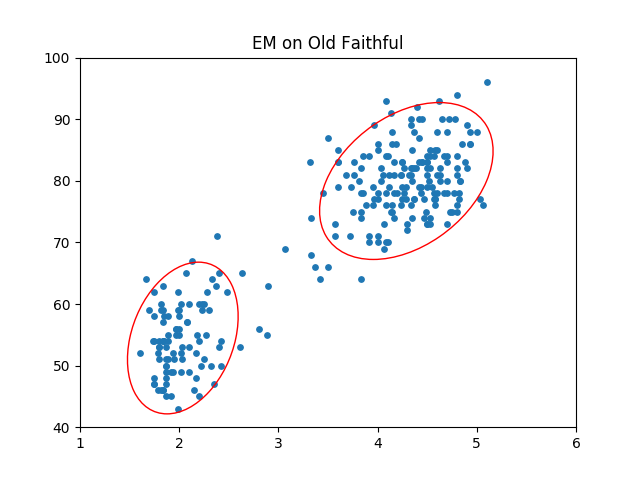
\includegraphics[height=2.3in]{exp-results/em_OF.png}}




\section*{Gibbs采样拟合GMM算法简述}
应用Collapsed Gibbs sampling拟合GMM模型的数学背景实在过于复杂,报告页数有限,我只着重描述算法的基本过程和直接相关的概率公式,对于其数学背景和正确性的证明可以参见Machine Learning-A Probabilistic Perspective一书。
\par 最核心的,Gibbs拟合GMM的算法是围绕着“每个观测样本最有可能来自哪个高斯分量”这一问题进行的。(实际上,这一点EM算法也是类似的,只不过是通过责任$\gamma$表现。)该模型中显示的引入一个N维向量$z$,$z_i$表示第i个观测样本属于哪个高斯分量,形成一个“硬分类”。

\subsection*{核心概率模型}
Gibbs拟合GMM做出的核心先验假设是:(1)各高斯分量的$\mu_k,\Sigma_k$独立,给定$\Sigma_k$,$\mu_k$服从正态分布,$\Sigma_k$则服从inverse Wishart分布。(2)$\pi_k$与$\mu_k,\Sigma_k$独立,服从Dirichlet分布。
\par 于是我们需要额外映入超参(作为先验一般是各高斯分量公用的):
\par 1. $\alpha$ \qquad  $\pi$的Dirichlet分布参数
\par 2. $m_0$ \qquad   $\mu$的先验高斯均值
\par 3. $\kappa_0$ \qquad $m_0$的可信度
\par 4. $S_0$ \qquad $\sigma$的先验IW参数
\par 5. $v_0$ \qquad $S_0$的可信度
\par 对于每个高斯分量,以$N_k$表示属于它的样本数量,维护一组后验参数:
\[\kappa_N = \kappa_0 + N_k\]
\[m_{N}=\frac{\kappa_0 m_0 +N_k \bar x}{\kappa_n} \]
\[v_N=v_0+N_k\]
\[S_N = S_0 + S_{\bar x} + \frac{\kappa_0 N_k}{\kappa_N}(\bar x - m_0)(\bar x - m_0)^T\]
其中$S_{\bar x}=\sum_{n=1}^{N}(x_n-\bar x)(x_n-\bar x)^T$
\par (不难发现当算法完成时,对于每个高斯分量,自己的$m_{N}$就接近类内样本的均值,$S_{N}$接近类内样本协方差的$N_k$倍。)
\par 忽略推导过程我们直接写出,某个样本属于第k个分量的概率(式子中所有参数表示拿掉第i个样本剩下的集合中第k个高斯分量对应的参数):
\[P(z_i=k|z_{/i},X,\alpha,m_0,\kappa_0,S_0,v_0) \propto P(z_i=k|z_{/i},\alpha)P(x_i|X_{k/i},m_0,\kappa_0,S_0,v_0)\]
\par 其中:
\[P(z_i=k|z_{/i},\alpha)=\frac{N_{k/i}+\alpha}{N+K\alpha -1}\]
\[P(x_i|X_{k/i},m_0,\kappa_0,S_0,v_0)=\pi^{-D/2}\frac{(\kappa_N +1)^{-D/2}{|S_N|}^{-(v_N+1)/2}\prod_{i=1}^{D}\Gamma(\frac{v_N+2-i}{2})} {(\kappa_N )^{-D/2}{|S_N|}^{-(v_N)/2}\prod_{i=1}^{D}\Gamma(\frac{v_N+1-i}{2})}\]
其中第二项也可以用等价的Student t distribution计算(两个方法在代码中都有实现,效果完全等价,但是后者计算速度要相对快一些)
\subsection*{具体算法}
给出了概率计算的公式以后,采用“采样”的方式实现拟合就比较顺理成章了。
\par 首先初始化z,即给每个样本指定开始属于哪个分量。
\par 每轮迭代,遍历样本,每取出一个样本(令其不再属于之前的高斯分量),根据之前给出的三个公式即可对于每个高斯分量计算出$P(z_i=k|z_{/i},X,\alpha,m_0,\kappa_0,S_0,v_0)$,这样我们就得到了属于每个高斯的概率,把这个离散的分布律归一化后,基于它抽样,给样本重新指定分量。
\par 迭代结束后,我们得到最终的z,此时就可以很方便的拟合相应的GMM的各项参数。(这个过程既可以把$m_N,S_N/N_k$当做对应高斯的均值和协方差,也可以像我代码中实现的一样,由于是硬分类的,直接在每个分量的类内做多元高斯的最大似然估计即$\mu=\bar x,\Sigma = \frac{1}{N_k-1}\sum_{x \in k}(x-\bar x)(x-\bar x)^T$,而$\pi=\frac{N_k}{N}$)

\par 我自己实现的算法中,我人为干预最后一次迭代,因为对于最后一轮迭代而言,实际上各分量“大局已定”,这时候抽样已经没有意义了,所以我人为在最后一次迭代中把每个样本都送入概率最大的类(或者取后几轮中这个样本抽样结果的众数),避免个别点进入不应该去的类,平白增大那个高斯分量的协方差估计。(当然这个小优化对于样本比较多的情况就不会有什么提升。对高斯分布的比较开,每个点除了最近的高斯,由其他分量生成的概率几乎为0的情况也没有需要。但是对样本较少,各个分量靠近的情况还是可以考虑添加的) 


\centerline{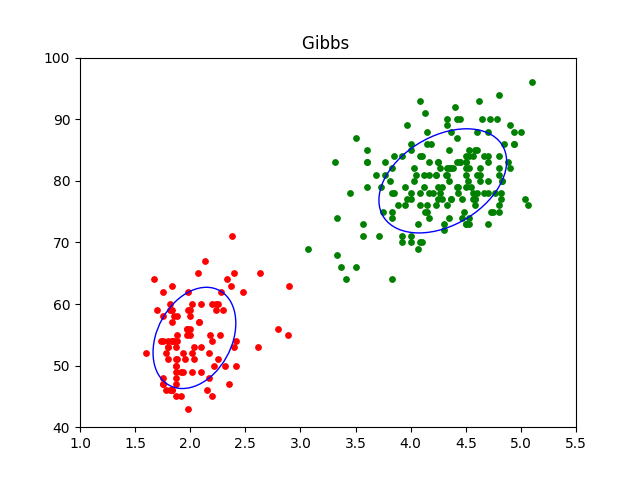
\includegraphics[height=2.4in]{exp-results/Gibbs_OF.png}}



\section*{对比实验及一些其他尝试}
\subsection*{数据生成} 
本次实验的数据除了引用了Old Faithful以外主要是通过自己定义的4个二维高斯,分别随机生成一些样本点,累加在一起形成(随机生成样本调用了numpy的multivariate\_normal),下面给出各个分量的参数,GMM的$\pi$可以认为有$\pi_k = N_k/N$\\
\begin{table}[!htbp]
% \resizebox{1.4\linewidth}{!}
  \centering
  \scalebox{1}{
\begin{tabular}{ l || c | c | c | c}
  \hline      
	component  & $\mu$ & $\Sigma$ & $N_k$  \\ \hline
	k=0  & (20,20) & ((25,0)(0,25)) & 150 \\
	k=1   & (60,40) & ((10,30)(5,30)) & 50 \\
	k=2     & (30,60) & ((10,5)(5,10)) & 100 \\
	k=3    & (40,40) & ((10,5)(5,10)) & 100 \\
  \hline  
\end{tabular}
}
\caption{生成样本参数}
\label{tb:lda_knn}
\end{table}

\subsection*{EM效果展示}
本次实验的数据上,随机选取个高斯分量均值,多数情况下的结果如下:\\
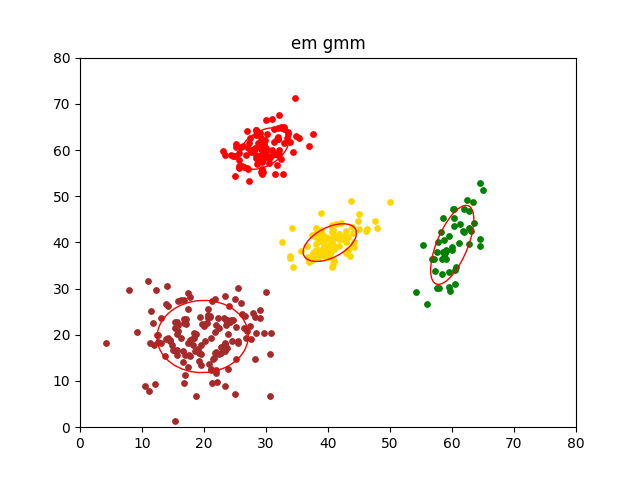
\includegraphics{exp-results/EM_rand4.png}\\
\begin{table}[!htbp]
% \resizebox{1.4\linewidth}{!}
  \centering
  \scalebox{1}{
\begin{tabular}{ l || c | c | c }
  \hline      
	component  & $\mu$ & $\Sigma$ & $\pi_k\%$  \\ \hline
	k=0  & (19.8,19.6) & ((27.0,0.6)(0.6,30.0)) & 37.50 \\
	k=1   & (60.0,39.4) & ((6.0,9.5)(9.5,36.5)) & 12.50 \\
	k=2     & (29.6,60.3) & ((8.2,3.8)(3.8,10.1)) & 25.00 \\
	k=3    & (40.2,39.9) & ((9.2,4.3)(4.3,8.3)) & 25.00 \\
  \hline  
\end{tabular}
}
\caption{EM拟合出的参数(顺序有所调整)}
\label{tb:lda_knn}
\end{table}\\
\\
\par 直观上看,不论是可视化后的结果还是具体的数据,结果都相当令人满意。尤其是,由EM迭代时$\pi$的估计公式,$\pi_k$作为“软分类”下第k个分量中样本数在总样本中的占比,最终收敛得尤其精确。同时多数情况下迭代迭代也在15次以内。(我以对数似然函数的变化小于1e-5为结束条件,对绝对值在1e3数量级的对数似然函数而言这个条件已经很严格了)
\par 如果一定要求定量的分析“准确率”,那么我认为对于均值可以对每个分量求$err(\mu)=\frac{\|\mu_{true} - \mu\|}{\|\mu\|}$,即误差向量的长度比上真实均值的长度,类似的$\pi$也可以比较误差率,但平心而论,这么做并无太大意义,基本上从图的可视化中我们就能清晰地感受到EM的任务已经完美的达成了。
\par 另一个相对可行的定量的指标是看算法结束后,同高斯分量产生的各个样本是否聚到相应的分量上,这种方法对之后的Gibbs采样显然非常合适,对于“软分类”的EM算法而言,我们也可以把它转化为硬分类,即对样本i找使得$\gamma(z_{ik})$最大的k。
\par 根据以上原则,转化为硬分类(分类结果用颜色可视化), EM算法分错了0个,有$100\%$的准确率。

\paragraph{}当然,EM算法很大程度上会依赖于初始化的结果,实际上EM是一个确定性的算法,一旦初始化的位置确定了,最后得到的局部最优解的位置也是确定的,与迭代的次数无关。所以某些情况下,EM会“失败”:\\
\centerline{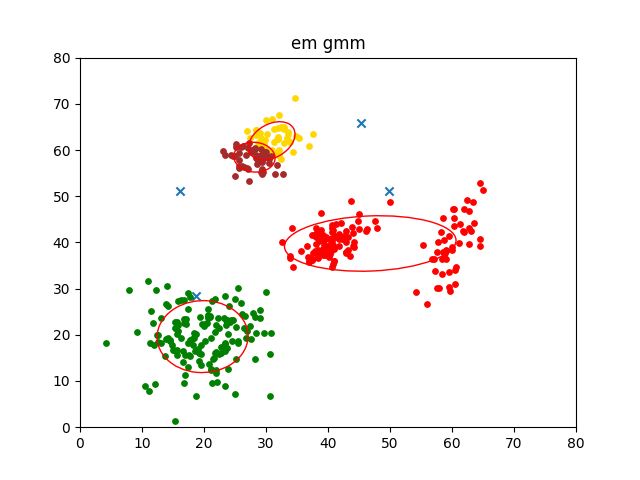
\includegraphics[height=3.5in]{exp-results/EM_fail.png}}
\par 叉表示初始化的均值位置,可以发现一个均值初始化在两类之间,两个均值初始化在离一簇点差不多距离的位置,造成了失败。


\subsection*{Gibbs效果展示}
\centerline{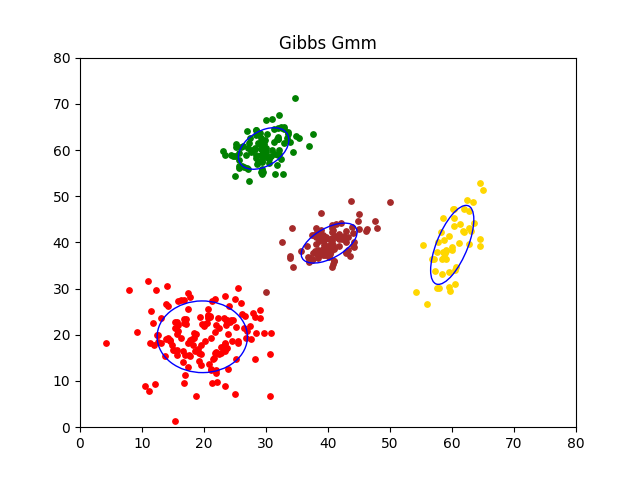
\includegraphics[height=3.5in]{exp-results/Gibbs_rand4.png}}
\par 同样,对绝大多数情况下,拟合的效果极佳,分类来看也只有一个点分错,而且这个唯一的小问题也是因为我关掉了上文提过的“小优化”,即最后一轮分类至概率最大的类而不是依照分布律抽样。(可视化已经足够说明问题了,不再做无谓的定量分析)
\par 迭代次数上来说,很多时候也在20次以内可以达成效果。
\par 虽然Gibbs同样非常受到初始化影响非常大,但从我的整个项目,近一周以来的大量的结果来看,相对而言Gibbs失败的概率要比EM小。
\par 少数失败的情况:\\
\centerline{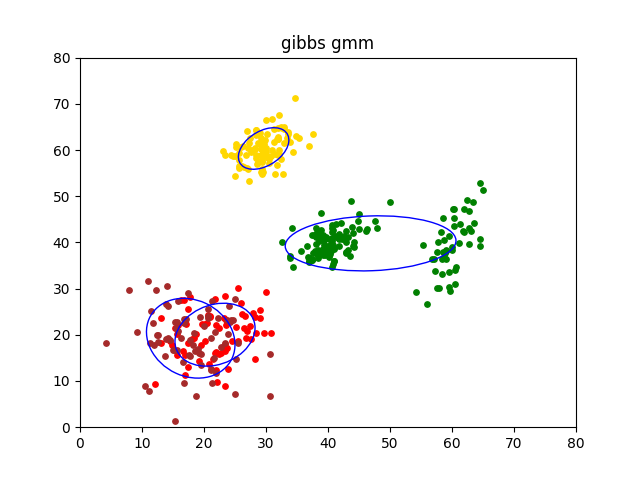
\includegraphics[height=3in]{exp-results/Gibbs_fail.png}}


\subsection*{样本数量的影响}
\par将之前的样本按照各个分量的比例等比例减少,各种情况运行10次,统计失败次数(可视化以后拟合是否成功其实相当直观,虽然没有量化,但也可以说是不含太多主观因素的)。

\begin{table}[!htbp]
% \resizebox{1.4\linewidth}{!}
  \centering
  \scalebox{1}{
\begin{tabular}{| l || c | c |}
  \hline      
	N  & EM & Gibbs  \\ \hline
	200  & 3 & 1 \\
	80   & 6 & 3  \\
	40   & 8 & 7  \\
  \hline  
\end{tabular}
}
\caption{样本数量对失败率的影响}
\label{tb:lda_knn}
\end{table}
\par
\par 分类效果展示,如果失败次数多于成功,则取分类失败时的图像。

\centerline{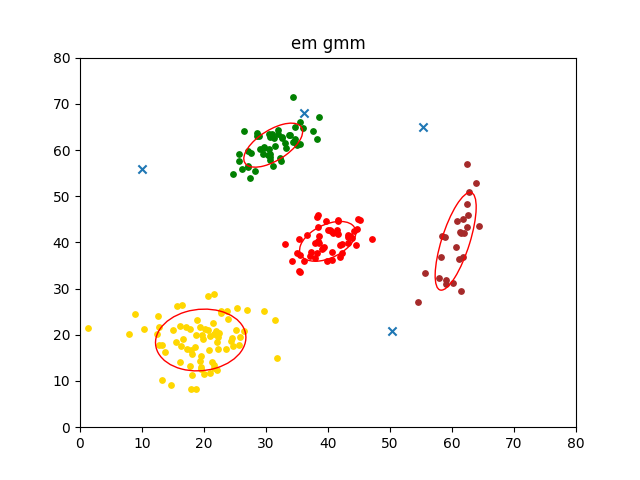
\includegraphics[height=2in]{exp-results/EM-200.png}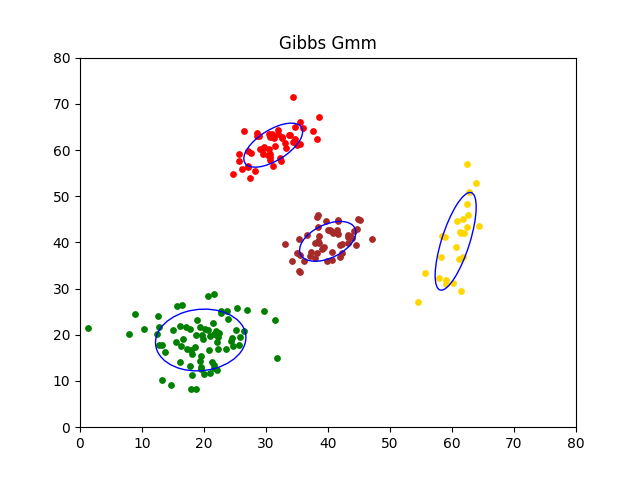
\includegraphics[height=2in]{exp-results/Gibbs-200.png}}
\centerline{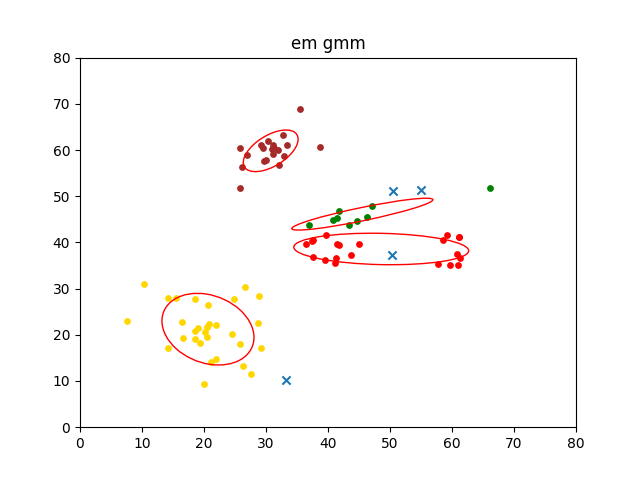
\includegraphics[height=2in]{exp-results/EM-80.png}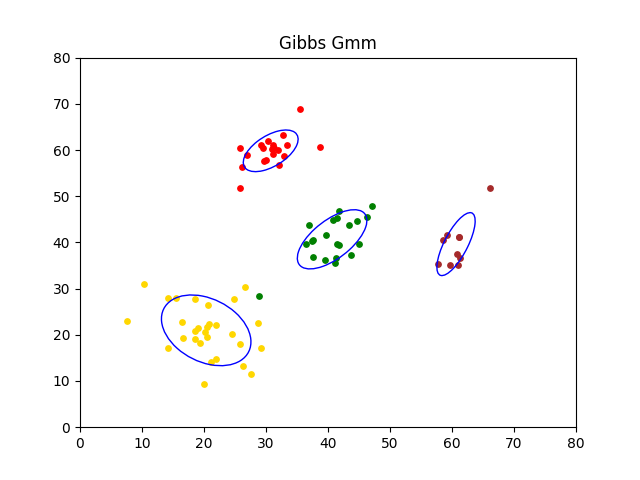
\includegraphics[height=2in]{exp-results/Gibbs-80.png}}
\centerline{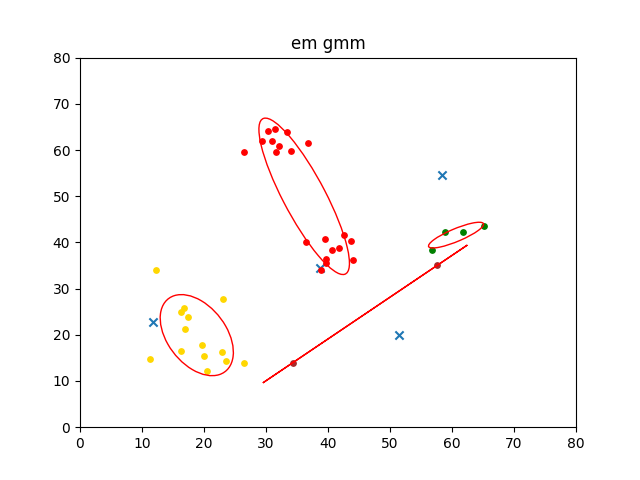
\includegraphics[height=2in]{exp-results/EM-40.png}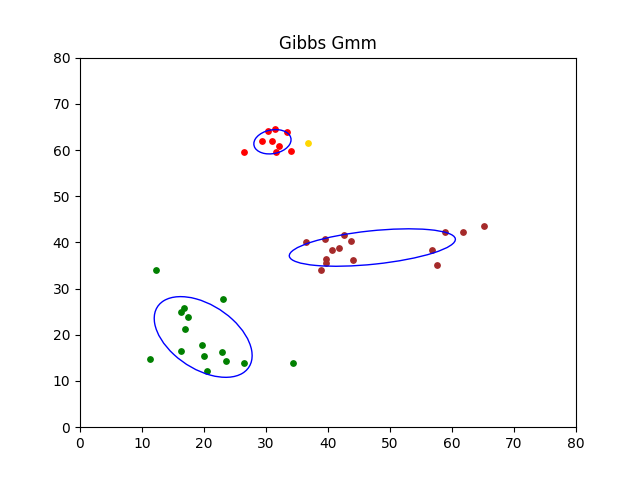
\includegraphics[height=2in]{exp-results/Gibbs-40.png}}

\par 可以看到当样本数量逐渐减少的时候,对于两种算法而言表现都在逐渐变差,这是因为虽然从人的主观上感觉,点越少图片越清晰,但是,一来实际生成样本时候各类的均值方差没有变化(各类样本并没有实质被拉开),二来有的类只有很少的样本就不能很好的表现这个相应高斯分量的特性,三来样本变少受别的高斯分量的样本的影响就变大。所以样本过少,不论是EM还是Gibbs效果都变得很差。
\par 同时,这个实验也验证了我之前的结论,就是相比较而言Gibbs算法的成功率更高,尤其是在样本较少(但不特别少)的情况下,这个看似主观的“成功率”的观测我觉得比同样成功拟合下的“准确率”有意义。

\subsection*{模型复杂度的影响}
\par 我理解的模型复杂度就是指定的拟合GMM的高斯分量数目K(之前的实验中,我们都指定了真实的分量数)。
\par 首先来看指定的高斯分量数少于真实值时的拟合效果:\\
\centerline{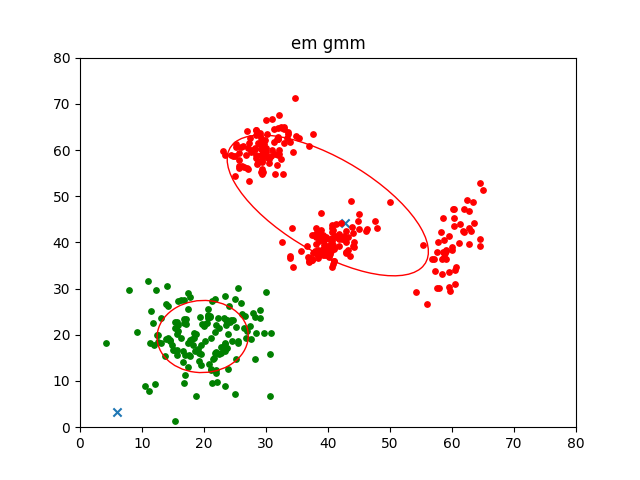
\includegraphics[height=2in]{exp-results/EM-2K.png}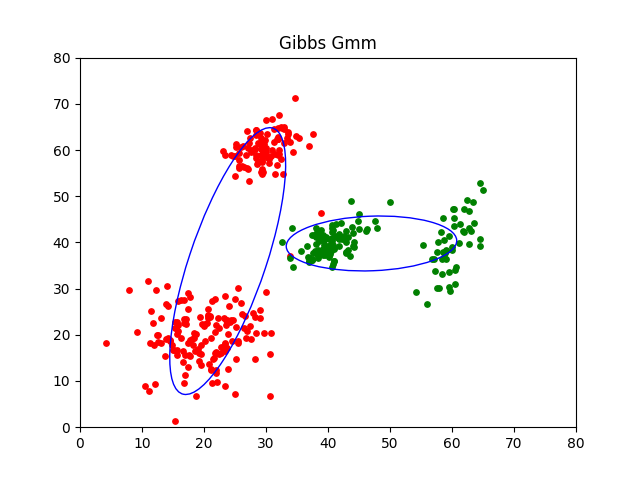
\includegraphics[height=2in]{exp-results/Gibbs-2K.png}}
\centerline{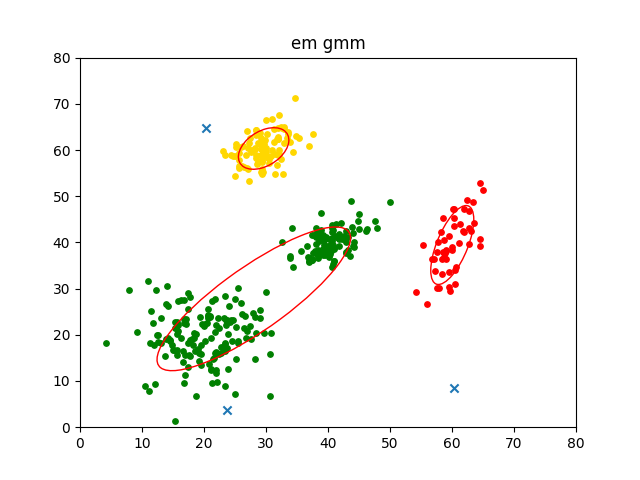
\includegraphics[height=2in]{exp-results/EM-3K.png}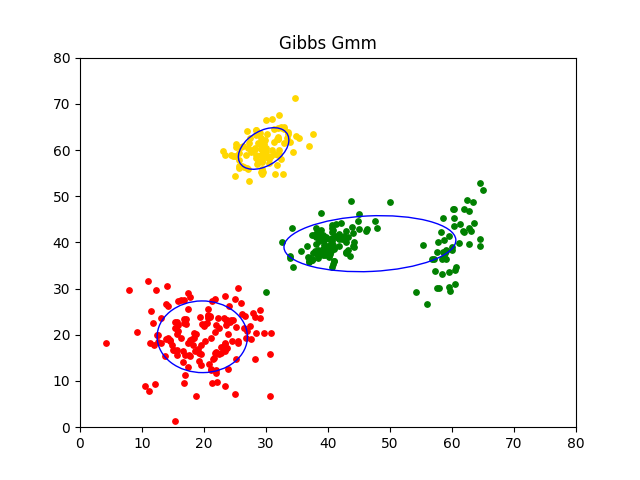
\includegraphics[height=2in]{exp-results/Gibbs-3K.png}}
\par 可以发现当指定的分量数少于真实值时,两种算法都表现出非常好的适应性,直观的来看,都是把部分的高斯合成了一组,并没有拟合到一些局部样本上,可以说是有限条件下非常合理的拟合结果了。
\par 而对于指定高斯分量数多于真实值时,要特别说明的情况是,我们之前上文讲的(也是实际实现的)Gibbs算法(简单版)是很难支持这一情况的,由于是硬分类,所以很容易出现某些分类出现一个样本也没有的情况,这个时候原始的算法显然就会崩溃。但是实际上真正会选择Gibbs采样应用于拟合GMM的场景,往往是对不确定高斯分量数的GMM进行拟合,其完整版算法和我们之前讲的略有不同,更为复杂,但会将无样本的类删去以做到自己拟合K这个参数。(很抱歉,我尚未实现这一算法。)
\par 而对于EM而言,指定高斯分量数多于真实值时,拟合表现的还是很稳定的。基本上只是多出的高斯分量瓜分掉一些样本而已。\\
\centerline{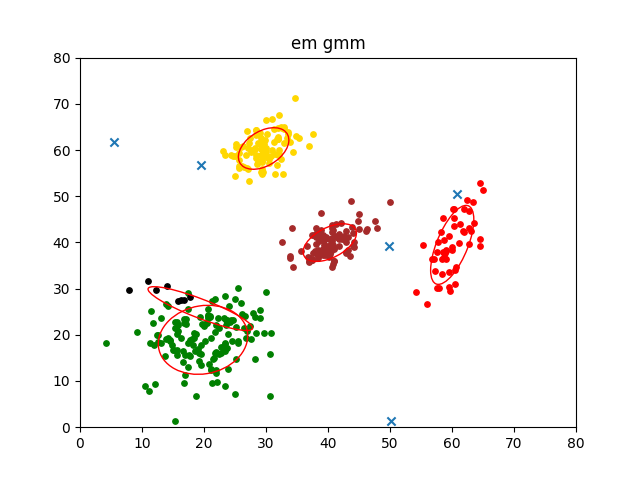
\includegraphics[height=2.2in]{exp-results/EM-5K.png}}
\subsection*{关于初始化}
\par 如前文再三强调的,两种算法都很大程度被初始化位置的影响。我自己的第一直觉是能不能尝试使用K-means聚类,对于EM算法而言是以把每个类的均值位置,作为EM算法中各高斯分量的均值,而对于Gibbs算法而言,K-means聚类的结果更是可以直接作为z的初始化。
\par 我使用K-means加EM做了实验,对于样本比较多,K正确的时候EM自身基本也是正确,但是这个时候K-means还是能有比较好的效果,那就是整个拟合过程的速度大大加快,K-means自身需要的迭代数目往往很少,而计算完成后,把均值交给EM,EM这时候基本只需要5轮以内的迭代就到达收敛的条件了。
\par 而对于样本较少的情况,我发现K-means并没有太大的提升EM的效果。仔细想来,虽然很多书上也建议使用K-means初始化EM拟合GMM的过程,但实际上对“准确性”不见得有很大提升,因为K-means自身也是非常依赖初始化的一种EM算法(实际上k-means,EM-GMM,Gibbs-GMM都存在着固定模型参数对样本分类,再对分完类的样本估计参数这样迭代的思想,三者非常类似)。所以K-means的主要贡献还是在于提速。
\par 但是在学K-means的过程中,我学习到一种初始化均值位置的小小优化,那就是随机均值的位置后,判断是否有两个均值里的较近,如果有则再次随机,这个做法的效果对样本较少的情况下,K-means+EM拟合GMM的最终效果有着不错的提升。\\
\centerline{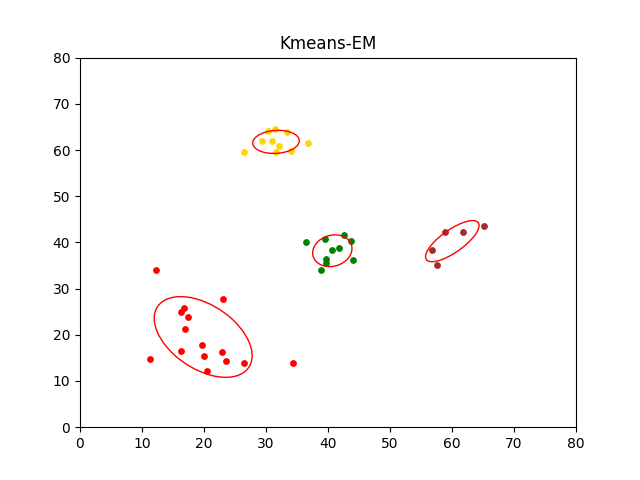
\includegraphics[height=3in]{exp-results/Kmeans-EM-40.png}}\\
\par 显然这个优化的假设是一般成立的,我们只要选择一个比较好的判断是否两个均值初始化位置过近的阈值即可。这个优化也可以脱离K-means直接使用在EM拟合GMM时的初始化过程中。

\subsection*{小结}
\par 总的来说,EM和Gibbs算法都是效果不错的拟合GMM的算法,两者虽然数学背景大相径庭,但是核心的思想有不谋而合,就是“根据现有参数估计样本来自哪个分量”和“根据各分量内的样本重新估计参数”的迭代。但是EM是一种软分类,Gibbs是一种硬分类。
\par 两者都很受初始化的影响,但EM是确定性算法,Gibbs是基于概率采样的,理论上后者更有可能跳过一个不好的局部最优解。
\par 从实践来看,在指定高斯分量数目正确的情况下,无论样本多少,Gibbs相对效果稳定。
\par 完整版的Gibbs可以用于高斯分量数目不确定的情况,EM则不行。
\par 迭代的速度上由于样本不多,没有明显的差距。


\subsection*{备注}
\par 本次实验的两种算法而定概率模型参考了PRML和Machine Learning-A Probabilistic Perspective。两个算法的主体部分在EM.py和Gibbs.py中实现,配有备注。使用的方法可以参考我在experiments.py中的代码(这部分代码由于我一直覆盖使用,所以并不涵盖所有报告中涉及的实验代码,也比较凌乱)。dataloader.py中是生成和载入数据的部分。使用的数据在data文件夹中。实验的很多结果在exp-results文件夹中。k-means的部分由于不是项目的重点基本仿照自github。
\par 实验中除了python自带的库,只使用常用的numpy和matplotlib



\bibliographystyle{plain}
\bibliography{report}


\end{document}